
Skip to content
Pull requests
Issues
Marketplace
Explore
@kamil271e
kamil271e /
embedded-systems-lab
Private

Code
Issues
Pull requests
Actions
Projects
Security
Insights

    Settings

embedded-systems-lab/lab1/Sprawozdanie.tex
@kamil271e
kamil271e Finished 1st report and added .gitignore
Latest commit e435998 1 hour ago
History
1 contributor
169 lines (154 sloc) 4.93 KB
\documentclass[polish,a4paper]{article}
\usepackage[utf8]{inputenc}
\usepackage[T1]{fontenc}
%%\usepackage{polski}
\usepackage{amsmath}
\usepackage{amssymb,amsfonts,amsthm}
\usepackage{babel}
\usepackage{hyperref}
\usepackage{xcolor}
\usepackage{graphicx}
\usepackage{caption}
\usepackage{subcaption}
\usepackage{listings}
\usepackage{anysize}
%%\usepackage{tabto}

\graphicspath{ {img/} }
\title{Arduino – układy wejścia/wyjścia (SW lab01)}
\author{Olga Gerlich 148088, Kamil Kałużny 148121 grupa I1.2}
\marginsize{2.5cm}{2.5cm}{0cm}{3cm}

\definecolor{codegreen}{rgb}{0,0.6,0}
\definecolor{codegray}{rgb}{0.5,0.5,0.5}
\definecolor{codepurple}{rgb}{0.58,0,0.82}
\definecolor{backcolour}{rgb}{0.95,0.95,0.92}

\lstdefinestyle{mystyle}{
	backgroundcolor=\color{backcolour},
	commentstyle=\color{codegreen},
	keywordstyle=\color{magenta},
	numberstyle=\tiny\color{codegray},
	stringstyle=\color{codepurple},
	basicstyle=\ttfamily\footnotesize,
	breakatwhitespace=false,
	breaklines=true,
	captionpos=b,
	keepspaces=true,
	numbers=left,
	numbersep=5pt,
	showspaces=false,
	showstringspaces=false,
	showtabs=false,
	tabsize=2
}

\lstset{style=mystyle}

\begin{document}
	\maketitle
	\section{Dobór rezystancji dla diody zielonej, żółtej i czerwonej}
	\subsection{Obliczenia rezystancji dla diód o różnych kolorach}
	Wzór na rezystancję diody:
	$$R = \frac{U_Z - U_D}{I_D}$$
	Obliczenia dla kolejno: czerwonej, żółtej i zielonej diody:
	$$R_R = \frac{5 - \frac{1.6 + 2.2}{2}}{20 \cdot 10^{-3}} = 155 \Omega$$
	$$R_Y = \frac{5 - \frac{2 + 2.3}{2}}{20 \cdot 10^{-3}} = 142.5 \Omega$$
	$$R_G = \frac{5 - \frac{3.7 + 2}{2}}{20 \cdot 10^{-3}} = 107.5 \Omega$$

	\subsection{Zadanie ,,blink''}
	\begin{figure}[h!]
		\begin{center}
			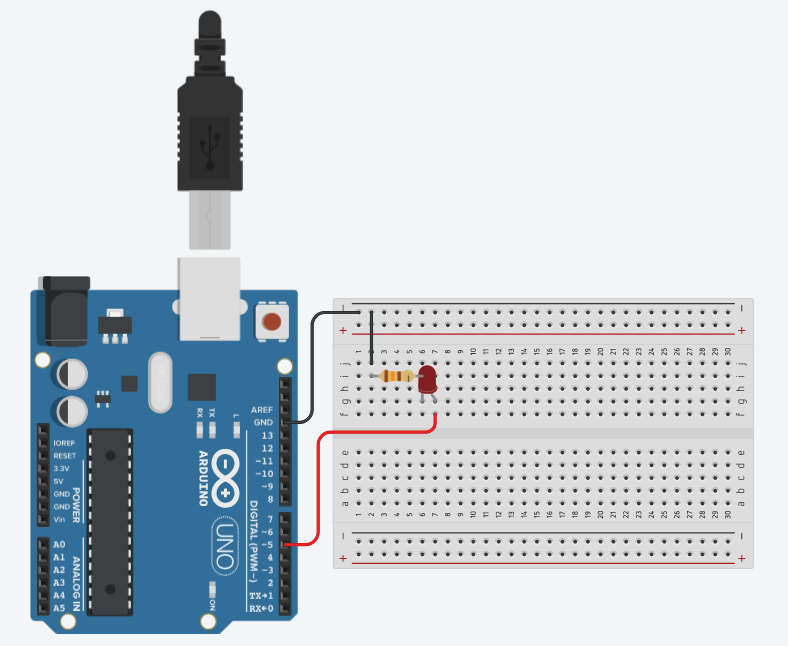
\includegraphics[scale=0.4]{01_blink.png}
			\caption*{Schemat podłączenia diody do Arduino}
		\end{center}
	\end{figure}
	\begin{figure}[h!]
		\begin{lstlisting}[language=C++]
			void setup() {
				pinMode(5, OUTPUT);
			}

			void loop() {
				digitalWrite(5, HIGH);
				delay(1000);
				digitalWrite(5,LOW);
				delay(1000);
			}
		\end{lstlisting}
		\caption*{Kod źródłowy}
	\end{figure}

	\newpage
	\section{Dioda + przycisk}
	\begin{figure}[h!]
		\begin{center}
			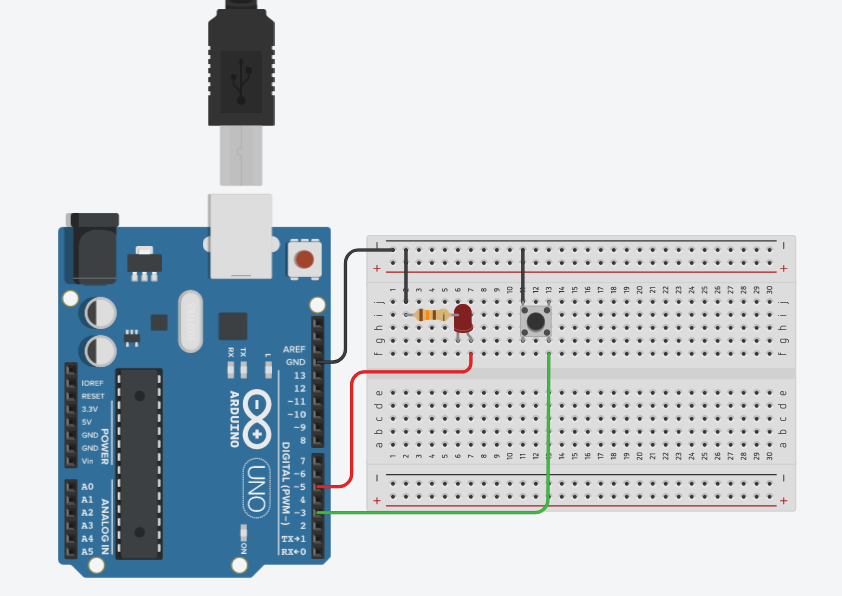
\includegraphics[scale=0.4]{02_button.png}
			\caption*{Schemat podłączenia diody oraz przycisku do Arduino}
		\end{center}
		\begin{lstlisting}[language=C++]
			int btn = HIGH;

			void setup() {
				pinMode(5, OUTPUT);
				pinMode(3, INPUT_PULLUP);
				digitalWrite(5, LOW);
			}

			void loop() {
				btn = digitalRead(3);
				if (btn == LOW){
					digitalWrite(5, HIGH);
				}
				else{
					digitalWrite(5,LOW);
				}
			}
		\end{lstlisting}
		\caption*{Kod źródłowy}
	\end{figure}

	\newpage
	\section{Potencjometr + dioda + Monitor Portu Szeregowego}
	\subsection{Zadanie ,,potencjometr i dioda''}
	\begin{figure}[h!]
		\begin{center}
			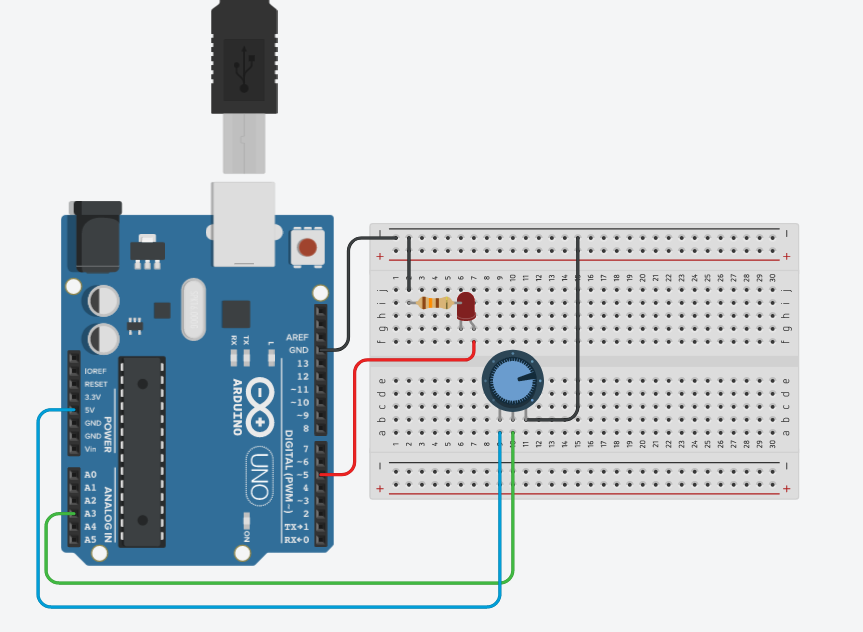
\includegraphics[scale=0.4]{03_serial_conn.png}
			\caption*{Schemat podłączenia diody oraz potencjometru do Arduino}
		\end{center}
		\begin{lstlisting}[language=C++]
			void setup() {
				pinMode(5, OUTPUT);
				pinMode(A3, INPUT);
				digitalWrite(5, LOW);
				Serial.begin(9600);
			}

			void loop() {
				Serial.println(analogRead(A3));
				if (analogRead(A3) >= 600){
					digitalWrite(5, HIGH);
				} else{
					digitalWrite(5,LOW);
				}
			}
		\end{lstlisting}
		\caption*{Kod źródłowy}
		\begin{center}
			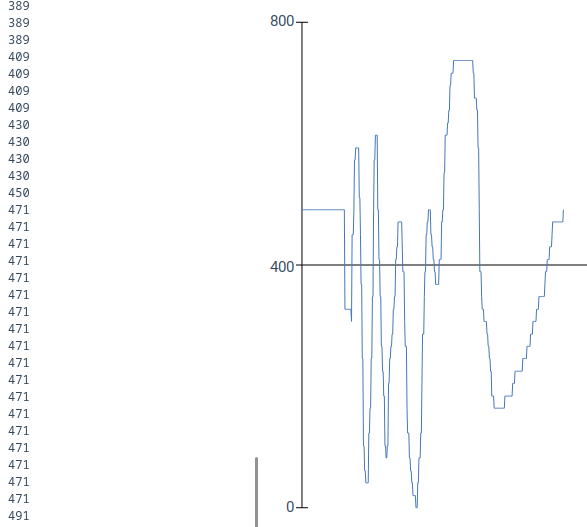
\includegraphics[scale=0.45]{Serial.png}
			\caption*{Zrzut ekranu z monitora portu szeregowego}
		\end{center}
	\end{figure}

	\subsection{Opis działania przetwornika A/C}
	%\tab
	 Przetwornik analogowo-cyfrowy zamienia ciągły sygnał analogowy na dyskretny sygnał cyfrowy.
	Są 3 etapy w procesie przetwarzania A/C próbkowanie, kwantowanie i kodowanie.
	\begin{itemize}
		\item \textbf{Próbkowanie} to pobieranie próbek analogowego sygnału co stały okres zwany okresem próbkowania. Im krótszy okres próbkowania tym dokładniejsze odwzorowanie zmian przebiegu wejściowego. Zbiór próbek musi być skończony, by można było go dalej przetwarzać cyfrowo.
		\item \textbf{Kwantowanie} odpowiada za konwersje, polega na ustaleniu pewnego zakresu oraz rozdzielczości skwantowanego sygnału cyfrowego, do którego przybliżane zostają określone wartości sygnału analogowego.
		\item \textbf{Kodowanie} jest procesem konwersji binarnej liczby, otrzymanej z procesu kwantowania, do innej, potrzebnej w danej chwili, postaci np. dziesiętnej.
	\end{itemize}

	\begin{figure}[h!]
		\begin{center}
			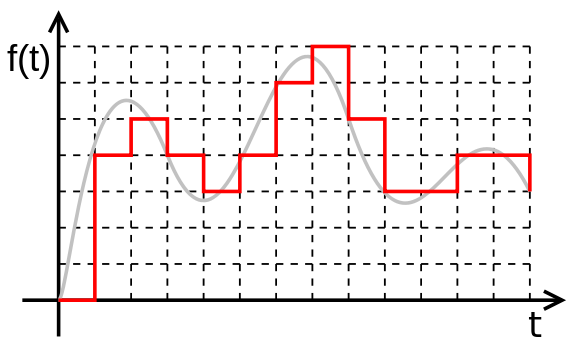
\includegraphics[scale=0.45]{Quant.png}
			\caption*{Wykres przedstawiający proces kwantowania}
		\end{center}
	\end{figure}

	\section*{Źródła}
	\begin{enumerate}
		\item \href{https://pl.wikipedia.org/}{Wikipedia}
		\item \href{https://agdlab.pl/slownik/Kwantowanie,171}{agdlab.pl}
	\end{enumerate}
	\begingroup
	\hypersetup{hidelinks}
	\tableofcontents
	\endgroup
\end{document}
Footer
© 2022 GitHub, Inc.
Footer navigation

    Terms
    Privacy
    Security
    Status
    Docs
    Contact GitHub
    Pricing
    API
    Training
    Blog
    About

embedded-systems-lab/Sprawozdanie.tex at main · kamil271e/embedded-systems-lab
